\documentclass[12pt]{article}
\usepackage[utf8]{inputenc}
\renewcommand{\familydefault}{\sfdefault}
\usepackage{graphicx}
\graphicspath{ {./} }
\usepackage[margin=1.2in]{geometry}

% For making the timeline:
\usepackage{pgffor}
\usepackage{tikz}
\usetikzlibrary{decorations.pathreplacing}

\usepackage{longtable} % To allow tables to cross pages
\renewcommand{\arraystretch}{1.5}  % Table padding

\hyphenpenalty=10000
\emergencystretch \textwidth
\usepackage[hidelinks,pdfusetitle,pdflang={en-GB}]{hyperref}


\title{Appendix~A: Elections, Appointments and Terms~of~Office}
\author{Van~Mildert~College Junior~Common~Room}
\date{26th June 2020}

\begin{document}
    \begin{titlepage}  % Title page
        \maketitle
        \begin{figure}[h]
            \includegraphics[scale=0.25]{arms}  % Coat of arms
            \centering
        \end{figure}
        \thispagestyle{empty}
    \end{titlepage}
    \setcounter{page}{2}  % Correct page numbering

    This appendix outlines the timings of elections, appointments and terms of office.\\
    (This appendix is advisory and summarises what is contained in the binding Standing Orders.)

    \section*{The Academic Year}
    The academic year runs from 1st August to 31st July.\\
    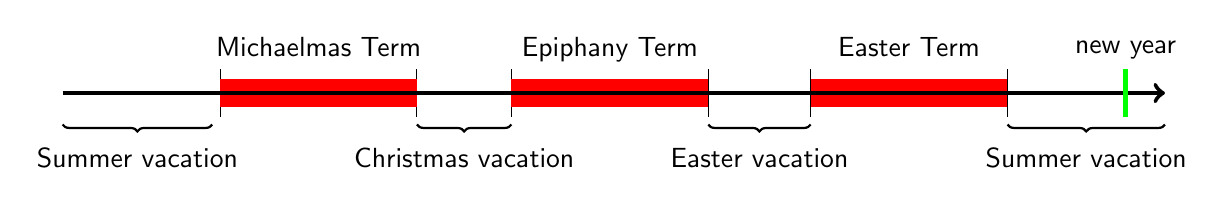
\begin{tikzpicture}
        \foreach \x in {2,4.5,5.7,8.2,9.5,12} {\draw (\x,.3) -- (\x,-.3);} % ticks
        % terms
        \foreach \x/\term in {2/Michaelmas,5.7/Epiphany,9.5/Easter} {
            \draw [red,line width=10] (\x,0) -- +(2.5,0)
                node [black,midway,above=5,text depth=0] {\term\ Term};
        }
        \draw[ultra thick, ->] (0,0) -- (14,0); % axis

        \draw[ultra thick,green] (13.5,-.3) -- (13.5,.3)
            node [black,midway,above=10,text depth=0] {new year};
        % holidays
        \draw[thick,decorate,decoration={brace}] (5.7,-.4) -- (4.5,-.4)
            node [black,midway,below=5] {Christmas vacation};
        \draw[thick,decorate,decoration={brace}] (9.5,-.4) -- (8.2,-.4)
            node [black,midway,below=5] {Easter vacation};
        \draw[thick,decorate,decoration={brace}] (14,-.4) -- (12,-.4)
            node [black,midway,below=5] {Summer vacation};
        \draw[thick,decorate,decoration={brace}] (1.9,-.4) -- (0,-.4)
            node [black,midway,below=5] {Summer vacation};
    \end{tikzpicture}

    Freshers Week is the week before Michaelmas Term.


    \section{Elections}
    \begin{longtable}{|l|l|l|}
        \hline
        \textbf{Position} & \textbf{Election} & \textbf{Term starts} \\
        \hline\hline
        \endhead
        \hline
        \endfoot

        Senior Freshers' Representative         & Michaelmas Term           & Epiphany Term \\
        Student Trustees                        & Michaelmas Term           & 1st February \\
        Senior Welfare Officer                  & Michaelmas Term           & Easter Term\footnote{Incoming must work with incumbent during Easter vacation} \\

        President                               & Epiphany Term             & Academic year \\
        FACSO                                   & Epiphany Term             & Academic year \\
        International Officer                   & Epiphany Term             & Easter vacation \\
        Communications Officer                  & Epiphany Term             & Easter Term \\
        Events Officer                          & Epiphany Term             & Summer vacation \\
        Formals and Experiences Officer         & Epiphany Term             & Summer vacation\footnote{Incoming must organise Mildert Day} \\

        Outreach and Fundraising Officer        & Easter Term               & Summer vacation\footnote{Incoming should appoint Outreach Directors and Executives prior to their term} \\
        Sports and Societies Officer            & Easter Term               & Summer vacation \\
        Chair                                   & Easter Term               & Summer vacation \\
    \end{longtable}


    \section{Appointed Officers}
    \subsection{Interviews}
    Each interview panel should include the Chair, the President, the incumbent and officers listed below.
    \begin{longtable}{|l|l|l|}
        \hline
        \textbf{Position} & \textbf{Interviews} & \textbf{Panel} \\
        \hline\hline
        \endhead
        \hline
        \endfoot

        Head of Mildert Day                     & Michaelmas Term
        & \begin{tabular}{l}Events Officer\\Formals and Experiences Officer\end{tabular}\\\hline
        Head of Decorations Committee           & Michaelmas Term
        & \begin{tabular}{l}Formals and Experiences Officer\\Internal Assistant Events Officer\end{tabular}\\\hline
        Deputy Chair                            & Michaelmas Term
        & \\\hline

        Webmaster                               & Epiphany Term
        & \begin{tabular}{l}FACSO\\Communications Officer\end{tabular}\\\hline

        Shop Manager                            & Easter Term
        & \begin{tabular}{l}FACSO\\FACSO-elect\end{tabular}\\\hline
        Senior DSU Representative               & Easter Term
        & \begin{tabular}{l}\end{tabular}\\\hline
        Assistant Events Officers               & Easter Term
        & \begin{tabular}{l}Events Officer\\Events Officer-elect\end{tabular}\\\hline
        Head of Ball                            & Easter Term
        & \begin{tabular}{l}Events Officer\end{tabular}\\\hline
        Head of VMCFS                           & Easter Term
        & \begin{tabular}{l}Events Officer\end{tabular}\\\hline
        DUCKtator                               & Easter Term
        & \begin{tabular}{l}Outreach and Fundraising Officer\end{tabular}\\\hline
        Outreach Directors                      & Easter Term
        & \begin{tabular}{l}Outreach and Fundraising Officer\end{tabular}\\\hline
        Heads of Talk and Support               & Easter Term
        & \begin{tabular}{l}Senior Welfare Officer\end{tabular}\\\hline
        Head of Technical Committee             & Easter Term
        & \begin{tabular}{l}FACSO\\FACSO-elect\end{tabular}\\\hline
        Head of Gym Committee                   & Easter Term
        & \begin{tabular}{l}FACSO\\FACSO-elect\end{tabular}\\\hline
    \end{longtable}

    \subsection{Terms of Office}
    \begin{longtable}{|l|l|l|}
        \hline
        \textbf{Position} & \textbf{Start} & \textbf{End}\\
        \hline\hline
        \endhead
        \hline
        \endfoot

        Head of Mildert Day & Appointment & End of Easter Term\\
        Head of Decorations Committee & Appointment & End of Easter Term\\
        Deputy Chair & Christmas vacation & End of Michaelmas Term\\
        Webmaster & Summer vacation & End of Easter term\\
        Shop Manager & Summer vacation & End of Easter term\\
        Senior DSU Representative & Summer vacation & End of Easter term\\
        Assistant Events Officers & Summer vacation & End of Easter term\\
        Head of Ball & Summer vacation & End of Easter term\\
        Head of VMCFS & Summer vacation & End of Easter term\\
        DUCKtator & Summer vacation & End of Easter term\\
        Outreach Directors & Summer vacation & End of Easter term\\
        Heads of Talk and Support & Summer vacation & End of Easter term\\
        Head of Technical Committee & Summer vacation & End of Easter term\\
        Head of Gym Committee & Summer vacation & End of Easter term\\
    \end{longtable}
\end{document}